\section{Estado del arte: ciencia de los datos}
\label{sec:state_dataScience}

\subsection{Introducción}
\label{subsec:state_dataScience_intro}

Las bases de datos NoSQL no es lo único que ha traído el ``Big Bang'' de la
información en Internet. De la misma manera que se hace evidente la necesidad de
poder almacenar toda ésta nueva información de manera eficiente, también lo hace
la necesidad de aprovechar y utilizar éstos datos de manera eficiente. A éstos
efectos, se ha ido gestando una nueva disciplina dedicada al estudio de nuevos métodos para generar información útil a partir de datos de
cualquier manera, a la que hoy se conoce como ``ciencia de los datos'', o en
inglés, \emph{data science}.

El primer uso del término data a 1966 cuando Peter Naur utilizó en 1966
porque no le gustaba el nombre de  ``ciencias de la computación'', y consideraba
este último más apropiado. Incluso hoy en día, aunque el término lleve usándose en su forma actual más de veinte
años, no existe ninguna definición formal sobre qué entraña exactamente, sino
que simplemente diferentes investigadores han aportado su opinión en
qué quiere decir el término. Chikio Hayashi (\cite{Hayashi1998}) la definió como
\emph{un concepto para unificar estadística, análisis de datos y métodos
  relacionados}, y Zhu et. al (\cite{Zhu2011}) la definieron de forma elegante
como \emph{una nueva ciencia cuyo objeto de estudio son los datos}. 


\subsection{Flujo de trabajo}
\label{subsec:state_dataScience_workflow}

Dentro de un proyecto de análisis de datos, existen una serie de pasos que en
conjunto, forman una manera de trabajar que dentro de las múltiples técnicas y
herramientas disponible, se ha estandarizado:

\begin{figure}[ht!]
  \centering
  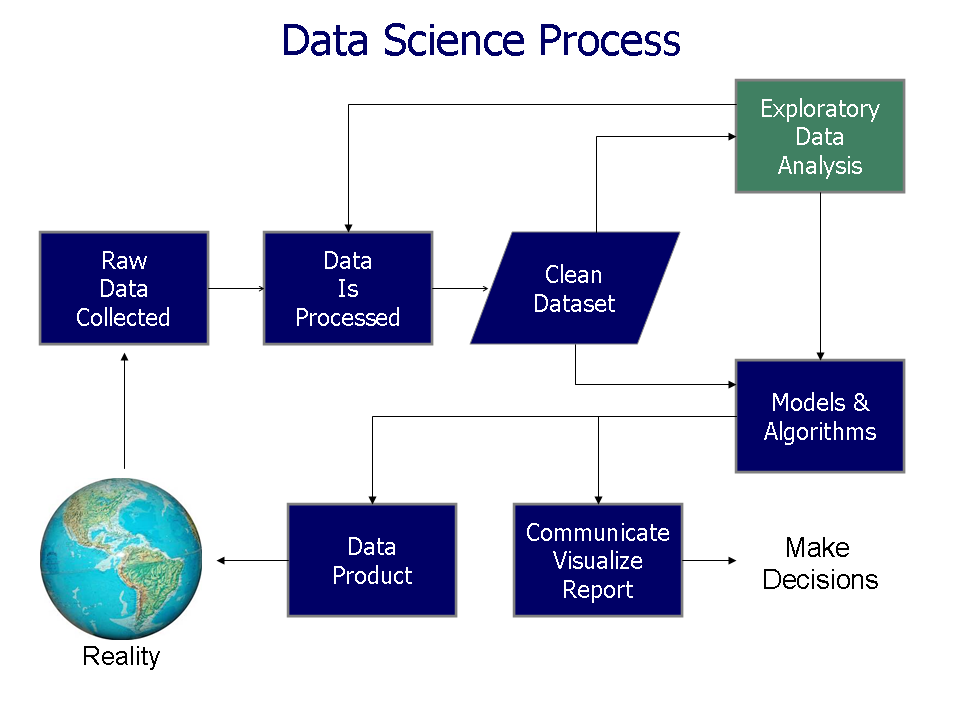
\includegraphics[scale = 0.65]{img/data_science_process.png}
  \caption{\label{fig:dataScienceWorkflow} Flujo de trabajo del científico de datos}
\end{figure}


\subsubsection{Formulación de la hipótesis}
\label{subsec:state_dataScience_workflow_1}

Al inicio del proyecto, nos encontramos ya de entrada con una decisión
importante. ?`Qué es lo que queremos investigar? ?`Con qué objetivo?

En un entorno corporativo, cada empresa operará en un mercado específico, y por
tanto, tendrá necesidades únicas. Es nuestra responsabilidad como parte de la
misma conocer bien las actividades de la misma, y los datos que genera, los
mismos sobre los que posteriormente realizaremos el análisis, y a partir de los
cuales generaremos un producto.

\subsubsection{Obtención de los datos}
\label{subsec:state_dataScience_workflow_1}

Una vez hemos decidido aquello que queremos definir, es hora de obtener los
datos. Éstos pueden venir de una infinidad de fuentes o formatos de fichero:
desde CSV, hojas de cálculo de Excel o LibreOffice y ficheros en formato JSON /
XML, a bases de datos relacionales y NoSQL. La siguiente tabla muestra la lista
de métodos de los que dispone Pandas (una librería para Python que provee
estructuras de datos y herramientas para facilitar el análisis) para leer
fuentes de datos, y generar un DataFrame (una estructura de datos tabular):


\begin{table}[h!]
\centering
\caption{Métodos de Pandas para leer datos}
\label{pandas_readData}
\begin{tabular}{|l|l|}
\hline
\textbf{Método} & \textbf{Fuente de datos}                                  \\ \hline
read\_csv       & Fichero CSV                                               \\ \hline
read\_excel     & Hoja de cálculo de Excel                                  \\ \hline
read\_hdf       & Fichero HDF (Formato de datos jerárquico)                 \\ \hline
read\_sql       & Base de datos relacional                                  \\ \hline
read\_json      & Fichero o cadena JSON                                     \\ \hline
read\_msgpack   & Formato de serialización msgpack                          \\ \hline
read\_html      & Tablas dentro de ficheros HTML                            \\ \hline
read\_gbq       & Google BigQuery                                           \\ \hline
read\_stata     & Ficheros DTA de Stata                                     \\ \hline
read\_sas       & Ficheros de SAS                                           \\ \hline
read\_clipboard & Contenidos del portapapeles a través de read\_table       \\ \hline
read\_pickle    & Estructuras de datos guardadas mediante el formato pickle \\ \hline
\end{tabular}
\caption{Métodos de Pandas para leer datos}
\end{table}

Obviamente, existen muchos más formatos en los que nos encontraremos los datos,
a parte de los que Pandas puede leer. En ese caso, nos tocará recurrir a más
herramientas mediante las cuales podamos interactuar con el servicio en
cuestión, para posteriormente transferir los datos a un DataFrame, o cualquier
otra estructura que deseemos utilizar.

% TODO: Hablar un poco sobre la minería de datos.

\subsubsection{Limpieza y preparación de los datos}
\label{subsec:state_dataScience_workflow_1}

Una vez ya hemos importado los datos, y los estamos manipulando con el lenguaje
de nuestra elección, debemos echarle un vistazo general al dataset, y ver si
observamos alguna anomalía.

En pandas, la clase DataFrame dispone de algunos métodos bastante interesantes
para ver rápidamente algunos registros del dataset: 

\vspace{0.5cm}

\begin{TMcode}{Python}{}{Bloque de código}
accidents_2015 = pd.read_csv("data/ACCIDENTS_GU_BCN_2015.csv", encoding="latin1", delimiter=";")

accidents_2015            # Muestra el dataset en su totalidad
accidents_2015.head()     # Muestra los 5 primeros registros
accidents_2015.tail()     # Muestra los 5 últimos registros
accidents_2015.sample(15) # Muestra 15 registros aleatorios
accidents_2015.describe() # Muestra diferentes métricas estadísticas sobre el dataset
accidents_2015.info()     # Muestra información sobre las columnas del dataset
\end{TMcode}

Por ejemplo, si ejecutamos \texttt{accidents\_2015.head()}, en una libreta de
Jupyter veremos lo siguiente:

\begin{figure}[ht!]
  \hspace{-0.7cm}
  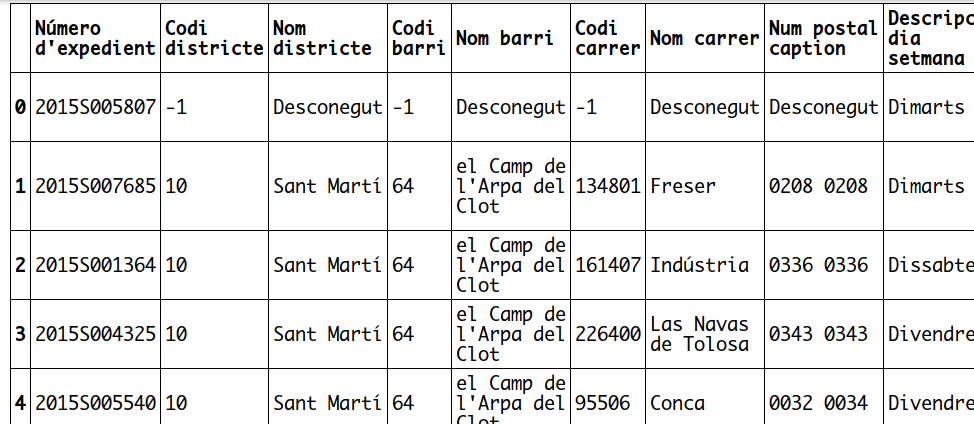
\includegraphics[scale = 0.45]{img/dataframeHead.png}
  \caption{\label{fig:dataframeHead} Dataframe.head() en Jupyter Notebook}
\end{figure}

Básicamente, las preguntas que deberíamos tratar de responder con éste análisis
inicial son las siguientes:

\begin{enumerate}
\item Existe alguna anomalía en los datos? Falta algún valor?
\item Observamos algún patrón en los datos?
\end{enumerate}


\paragraph{Trabajando con valores faltantes} \mbox{}\\

En caso de que en nuestro dataset nos encontremos con variables para las que
directamente no exista una observación, existen varias técnicas que podemos
utilizar para tratar los registros.

Las dos primeras que describiremos, trabajan de forma destructiva, es decir,
borrando datos: 

\begin{TMbulletin}{critical}{$¡$Aviso muy importante!}
  Al borrar / ignorar la informacion faltante, éstos métodos pueden
  introducir \textbf{imparcialidad estadísticaI}\footnote{Se da cuando
el resultado obtenido difiere del verdadero parámetro siendo estimado.}
\end{TMbulletin}

\begin{enumerate}
\item Borrar el registro entero en el qual falte alguna observación.
\item Ignorar observaciones faltantes, y realizar análisis únicamente sobre
  aquellas observaciones que sí se encuentren en el dataset.
\end{enumerate}

La otra manera de tratarlos recibe el nombre de \textbf{imputación}, y no es ni
más ni menos que la sustitución de los valores nulos. Para ésto, también
disponemos de varias técnicas:

\begin{enumerate}
\item Para variables contínuas, podemos sustituir valores nulos por la media
  aritmética de los valores no nulos.
\item Para variables categóricas, podemos sustituir valores nulos por la moda de
  los valores no nulos. El valor que más veces se dé, será el que utilizaremos
  en la imputación.
\end{enumerate}




\subsubsection{Análisis explorativo}
\label{subsec:state_dataScience_workflow_2}

\subsubsection{Modelado}
\label{subsec:state_dataScience_workflow_modeling}

\subsubsection{Comunicación de los resultados}
\label{subsec:state_dataScience_workflow_communication}

\subsubsection{Producto de datos}
\label{subsec:state_dataScience_workflow_dataProduct}





